\documentclass{ximera}

%% You can put user macros here
%% However, you cannot make new environments

\listfiles

\graphicspath{{./}{firstExample/}{secondExample/}}

\usepackage{tikz}
\usepackage{tkz-euclide}
\usepackage{tikz-3dplot}
\usepackage{tikz-cd}
\usetikzlibrary{shapes.geometric}
\usetikzlibrary{arrows}
\usetikzlibrary{decorations.pathmorphing,patterns}
\usetkzobj{all}
\pgfplotsset{compat=1.13} % prevents compile error.

\renewcommand{\vec}[1]{\mathbf{#1}}
\newcommand{\RR}{\mathbb{R}}
\newcommand{\dfn}{\textit}
\newcommand{\dotp}{\cdot}
\newcommand{\id}{\text{id}}
\newcommand\norm[1]{\left\lVert#1\right\rVert}
 
\newtheorem{general}{Generalization}
\newtheorem{initprob}{Exploration Problem}

\tikzstyle geometryDiagrams=[ultra thick,color=blue!50!black]

\usepackage{mathtools}



\title{Modeling a spring-mass system}
\author{Anna Davis, Just Greenly, , L. Felipe Martins, Paul Zachlin}

\begin{document}

\begin{abstract}
This lab describes an activity with a spring-mass system, designed to explore concepts related to modeling a real world system with wide applicability.
\end{abstract}


\maketitle

The goals of this project are:
\begin{itemize}
    \item Deepen your understanding of linear second order homogeneous differential equations.
    \item Study a prototype model application for the harmonic oscillator, via a spring-mass system.
    \item Practice with data collection, analysis and interpretation.
\end{itemize}

For this lab you will need:
\begin{itemize}
    \item A ``spring''. This can be a real spring, or, as a substitute, you can use a rubber band, or several smaller bands tied together.
    \item A ``mass''. The mass could be a roll of coins, a coffee mug (don’t use your favorite one), a stapler, a can of food, or any attachable small dense object.
    \item Measuring devices: a measure tape for measuring distances, and a kitchen scale to measure masses. A timing device, such as a smart phone. A regular watch may be hard to use. You will have to decide which units to use, and adjust all constants accordingly.
    \item (Optional) A video-recording device, such as a video camera, cell phone or tablet.
\end{itemize}

\section{Introduction}

The spring-mass system is good model problem, since there are many related application problems for which the same mathematical equations apply.  

This activity will instruct you on how to measure and model your own system, connecting the physical behavior of the model system with the mathematical features first introduced in Chapter 5 of Trench’s text.



Figure $\ref{fig:spring-mass-system}$ below demonstrates the situation when the mass is hung on a spring of length , stretching it by a distance   Any movement of the mass can be measured from this equilibrium position.  We make the arbitrary choice to call the upward direction positive, as noted in the figure.  

\begin{figure}
    \centering
    \begin{image}
    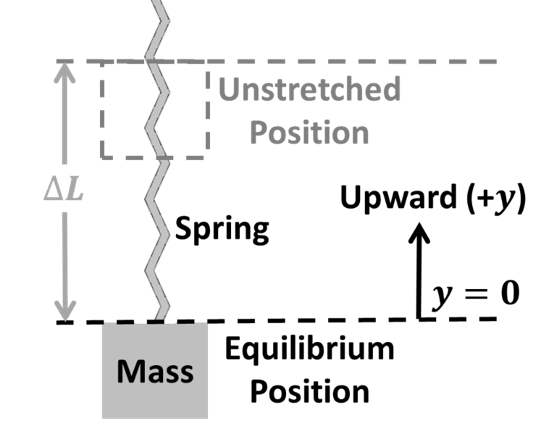
\includegraphics[scale=0.5]{spring-mass.png}
    \end{image}
    \caption{A spring-mass system}
    \label{fig:spring-mass-system}
\end{figure}

To set up the system, the spring should hang from above by some fixture such as a hook. Place the spring near a wall, and attach the measuring tape behind the spring. If using a recording device, set it up some distance away, in such a way that both the spring-mass system and the measuring tape are visible. The image below illustrates a possible setup.

\section{Model for the spring-mass system}

The model for the spring-mass system has the following parameters:
\begin{itemize}
    \item The mass, $m$.
    \item The relaxed length of the spring, $L$.
    \item The spring constant, $k$.
    \item The acceleration of gravity $g$.
    \item The coefficient of friction $c$.
\end{itemize}
The dynamic variable in the model is the displacement from the equilibrium position, which we denote by $y$. We assume that $y$ is positive in the upward direction.

In this first exploration, we assume that the friction is negligible. That is, as a first approximation, we assume that $c=0$.

Recall that we model the intensity of the force exerted by the spring by Hooke's law:
\[
|F_{\text{spring}}|=k\cdot\text{(spring deformation)}
\]
where the spring deformation is represented by $\Delta L$ in Figure~\ref{fig:spring-mass-system}. 

Using this information, answer the following questions:

\begin{problem}
What is the force on the spring due to gravity?
\[
\begin{prompt}
F_G=\answer{mg}
\end{prompt}
\]
\end{problem}

Let's now denote by $y_R$ the $y$-coordinate corresponding to the relaxed spring.

\begin{problem}
Using the fact that the total force at the equilibrium position is zero, determine an expression for $y_R$:
\[
\begin{prompt}
y_R=\answer{-mg/k}
\end{prompt}
\]
\end{problem}

\begin{problem}
What is the force exerted by the spring if the mass is at a generic position $y$?
\begin{prompt}
\[
F_S=\answer{-k(y+mg/k)}
\]
\end{prompt}
\end{problem}

\begin{problem}
Assuming that the coefficient of friction $c$ is zero, what is the total force, $F_T=F_R+F_G$ acting on the spring? Simplify your answer as much as possible.
\begin{prompt}
\[
F_T=\answer{-k y}
\]
\end{prompt}
\end{problem}

Newton's Second Law states that:
\[
\text{(mass)}\times\text{(acceleration)}=\text{(total force)}
\]

\begin{problem}
Use Newton's Second Law to find a differential equation for the acceleration of the mass:
\[
y''=\answer{-\frac{k}{m} y}
\]
\end{problem}

\begin{problem}
Find the general solution of this differential equation. Use $c_1$ and $c_2$ for the constants of integration.
\[
y(t)=\answer{c_1\cos\left(\sqrt{\frac{k}{m}}\right)+c_2\sin\left(\sqrt{\frac{k}{m}}\right)}
\]
\end{problem}

\begin{problem}
In the experiments we will perform, we will stretch the spring to a prescribed position $y_0$ and then let it go. This corresponds to the initial conditions $y(0)=y_0$ and $y'(0)=0$. Find the solution of the differential equation that corresponds to this situation.
\[
y(t)=\answer{y_0}\cos\left(\sqrt{\frac{k}{m}}\right)
\]
\end{problem}

\section{Running the experiment with the system}

Now set up the experiment. As an initial goal, let's try to establish the period of the oscillation.



\section{Spring in Equilibrium Position Stretched by Mass}

%Before we employ Physics to construct a model for the motion of this mass on a spring, take a minute to consider what would happen if we pulled the mass down a bit further and then released it.  
%•	How will the position of the mass change as a function of time?  
%•	Can you make a sketch of this motion (position vs. time)?  Try to make a sketch.
%•	What type of elementary function might best describe the motion?  
%o	Exponential, Linear, Quadratic or other Polynomial, Trigonometric, Logarithmic, or something else?
%•	Describe the distances and key features of your sketch with as much detail as possible.
%•	Will the motion continue indefinitely or will certain features change over time?
%Newton’s 2nd Law states that the sum of the forces acting on a body, otherwise known as the net force, will equal the mass of that body times the acceleration it experiences:
%
%This means that if all of the forces acting on the mass are quantified and the mass is known, it’s acceleration can be found.  This important equation from Physics will lead directly to a differential equation which can then be solved.  Recall that acceleration is the second derivative of position with respect to time.  We will use the convention that “up” is positive consistently as we account for forces and motion.  Force and acceleration are in bold because they are vector quantities that can account for multiple directions.  However, we will only consider one dimension of up and down in our analysis.  
%One force always acting on the body is the force of gravity, which acts downward and is equal to the mass  times the gravitational constant  (which is about ).  This force is also simply called the weight.  We will need to estimate the weight of the mass you have chosen to use.    
%Mass of object ():
%Weight of the mass (): 
%Another force acting on the body is the upward pull by the spring.  Hooke’s Law states that this force will be equal to a “spring constant” which we call  multiplied by the amount the spring is stretched.  This means that the force of the spring will be linearly proportional to the amount of stretch it experiences at any time.  The units of the spring constant are force per length such as .  We can find the amount of stretch by measuring the distance from the unstretched position of the bottom of the spring (with no mass attached) to its equilibrium position where the mass is hanging motionless from the spring.  This is the distance between the two dashed lines in the diagram above.  Use a ruler or meter stick to measure the length that the spring stretches due to the weight of the mass.  Be sure to measure consistently at the bottom of the spring.
%Distance of stretch: 
%Spring constant ():  
%When the mass is hanging motionless from the spring, the weight of the mass (acting downward) and the force of the spring (acting upward) are equal in magnitude and opposite in direction.  
%	
%Because these forces cancel each other exactly, Newton’s 2nd law shows that the acceleration of the mass is zero.  We say that the mass is at equilibrium.  We can now consider any changes relative to this equilibrium position.
%If the mass is moved downward any further, the spring stretches.  The spring will then pull upward with more force on the mass.  Since movement downward (in the negative  direction) causes this force to act upward, this additional force is .  The two negatives will cancel, given a positive number, which – by our convention – is upward.  
%If the mass is moved upward, the spring is compressed.  The spring would push downward on the mass.  Since movement upward (in the positive  direction) causes a spring force downward, the additional force is again .  
%If the mass is released with a non-zero initial position, the spring will oscillate due to this alternating force which always seeks to move the mass back towards the equilibrium position.  The restoring force would always accelerate the mass in the direction of the equilibrium position, but the mass would then develop enough velocity to pass this position and move an equal distance beyond it.  If there were no air resistance or dissipation of energy (sometimes known as dampening), the system would oscillate forever.  We will neglect dampening for now.
%As noted above, the two forces  and  will always cancel each other, leaving only the additional force .  Newton’s 2nd Law says that 
%
%Since acceleration is the second derivative of position with respect to time, this results in the following second order homogeneous linear differential equation:
%
%This can be rearranged into a standard form:
%
%The solution of this differential equation is:
%
%Do you remember how we find this solution?  If not, re-read section 5.2 of Trench’s book.  To confirm that it works, plug it back into the differential equation to check it.  To do this, you will need to take the first and then the second derivative of the solution.  Notice how the second derivatives of both trigonometric functions involve the negative of themselves and that the chain rule will “bring out” the square root term twice.  These attributes of the solution are necessary to make this differential equation true.
%If the initial position of the mass is recorded at  and it is released with no initial velocity, only the first term – the cosine term – in this equation is kept because the second constant will be zero.  
%The quantity  is referred to as the circular frequency, and has units of radians per second.  Taking this value and dividing by 2 gives the frequency in Hertz (Hz) which means cycles per second.  The inverse of this quantity in Hertz is the period of the motion, which is the time in seconds for one complete cycle.
%Use your measured quantities for your specific system, forming and solving the differential equation as above.  Compare your estimate of the period to the actual result by measuring the time the mass takes to oscillate through at least one cycle.  You will make a more accurate measurement if you record the time needed to complete three or more cycles.
%An Example from the Kitchen
%I don’t happen to have a nice long spring available, so I’ll use a long rubber band with a small can of cream of mushroom soup.  The can is labelled as containing or (), which we can use as an estimate of the mass.  To find the weight, we can multiply  by , giving .  I measure the length of the stretch of the spring to be  or .  The spring constant  is .  Calculating the  term as , the differential equation becomes:
%
%This has a solution 
%
%If I pull the can down  and release it with no initial velocity, two constants can be shown to be  and , respectively.  The first number comes from the initial position and the second comes from the initial velocity.  It is necessary to differentiate this equation once before applying the second initial condition that effectively says .  The final undamped solution becomes
%
%(insert graph here)
%The period of this motion predicted by the model is .  In my experiment at home, I estimated the period to be about .  This is a reasonable match.  However, I did note that with the rubber band, the motion dampens out significantly from its initial amplitude of around  after the first few cycles.  Our choice to ignore air resistance and energy dissipation is clearly unreasonable, even though the period of the motion predicted by the model seems like a decent match for the period in the real system.
%(insert embedded Ximera calculations to check students math and plot motion for inputs of m,  , and initial positions)
%
%
%(follow-up exercise with damping?)
%
%
%
%
%
%

\end{document}
